\section{ Motivation}

As a result of increasing human population and habitat loss, human-wildlife conflicts have become increasingly common in the last several decades\cite{philip-wildlife}.
According to the organization The World Wide Fund for Nature (WWF), human-wildlife conflicts are defined as: "any interaction between humans and wildlife that results in negative impacts on human social, economic or cultural life, on the conservation of wildlife populations, or on the environment"\cite{conflict-manual}.
These conflicts range from mostly harmless, non-violent contacts, such as sightings of wildlife animals in urban areas, to the destruction of crops and infrastructure, killings of livestock, and in the worst cases, losses of human lives.
In more severe cases these conflicts end in defensive or retaliatory killings of wildlife animals which can drive already endangered species to extinction.

Polar bears, tigers, and elephants are generally considered to be the most problematic \cite{philip-wildlife}.
In the Arctic, as a consequence of the reduction of their natural habitat, polar bears are drawn to human settlements, food dumps, while searching for food\cite{wildlabs-polarbears}.
Unexpected encounters can turn deadly for both sides.
As wide-ranging animals, tigers need large areas where they can roam, hunt, and breed\cite{wildlabs-tigers}.
When their natural prey population is depleted, they often turn their attention to poorly protected livestock. 
Their attacks often have economic, social, and psychological consequences.
According to WILDLABS, tigers killed 101 people between the years 2013 and 2016, in India alone\cite{wildlabs-tigers}.

As herbivores, elephants might be seen as less problematic when compared to polar bears or tigers, but this assumption could not be further from the truth.
Although exact numbers vary between sources, casualties from human-elephant conflicts (HEC) are much higher compared to conflicts involving polar bears or tigers.
According to WILDLABS, an average of 400 people and 100 elephants are killed every year in India\cite{wildlabs-elephants}. 
The leading cause of death of elephants is electrocution (by electric fences, unprotected power lines), followed by train accidents, poaching, and poisoning\cite{cause-of-death}.
One of HEC hotspots is in Sonitpur District, Assam province, India. 
In 5300 km\textsuperscript{2} large area around 200,000 people and 200 elephants share the same space\cite{wildlabs-elephants}.
Elephants often venture into paddy fields which represent livelihood for local communities.
A single elephant can quickly trample fields of rice crops in a few hours, causing big financial problems to already impoverished farmers\cite{wildlabs-elephants}.

Several measures have been taken to minimize HEC: electrical fences, watch towers, trenches, chilli-based deterrents, regular patrols, usage of trained captive elephants and camera traps with motion sensors.

Although the above mentioned measures function to some degree, they are not effective enough, since they are unreliable or come into effect when the damage has already been done\cite{wildlabs}. 

\section{ Early detection system}

One important component of minimizing human-elephant conflicts is a reliable early detection system. 
A system capable of detecting the presence of nearby elephants would warn nearby communities and give them enough time to prepare and respond nonviolently.
The same kind of system would also provide information about common elephant paths, thus giving farmers knowledge on how to better construct and place their fences to minimize HEC.
The system (Figure \ref{early_detection_system}) should consist of several small, deployed devices with mounted cameras, that will detect elephants and one server which will aggregate alerts and forward them to mobile phones, computers, where the local community will see them.

\begin{figure}[ht]
        \centering
        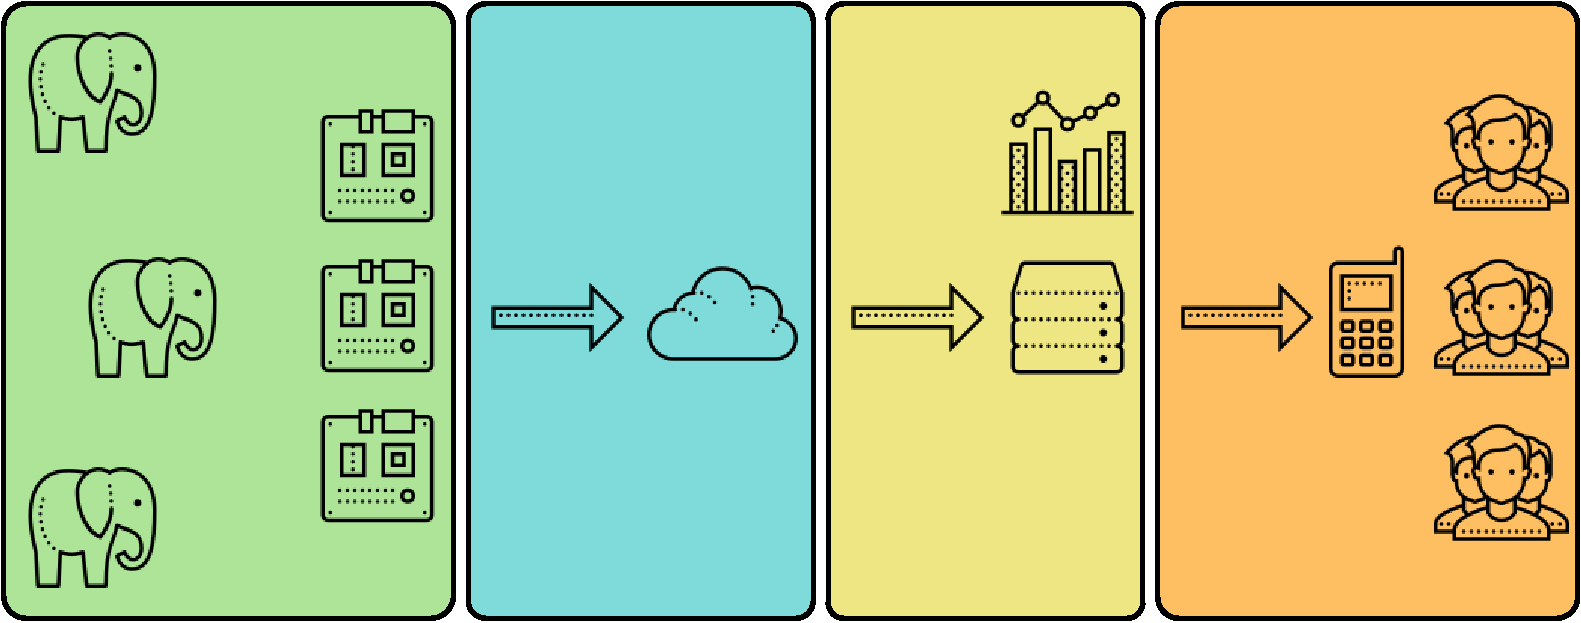
\includegraphics[width=1.0\linewidth]{early_detection_system.pdf} 
        \caption{Diagram of early detection system. Icons source: www.icons8.com}
        \label{early_detection_system}
\end{figure}

Although most of the villages in Sonitpur district have access to cell phones and the internet, the connectivity can be unreliable\cite{wildlabs-elephants}. 
Furthermore, devices will be placed quite far from the main server, which makes sending a large amount of data a problem. 
This limits choice of wireless networks to long range, low bandwidth technologies.
It is therefore preferable that elephant detection is done on deployed devices and only results (which can be big few bytes) are sent over some radio network to the main server.
Deployed devices will be placed in forests, fields, with no access to electricity, therefore they need to be battery powered.
Low maintenance of deployed devices is a desirable quality, which means that they should be functional for longer periods without any human interactions.
To achieve that with a limited power source, they should be energy efficient, equipped with solar panels, and a low power radio.
Devices should spend most of their time in sleep mode, conserving energy, only waking up to take a photo, processing it, and sending results to the main server.
As most of the human-elephant conflicts happen during night\cite{wildlabs-elephants}, a thermal camera is needed.

Elephant recognition can be done with the help of a convolutional neural network (CNN) running inference on a microcontroller. 
Making this possible and evaluating the solution is the focus of this master's thesis.


\section{ IRNAS and Arribada Initiative}

The system described above is currently in development at IRNAS in collaboration with Arribada Initiative.
Slovenia based Institute IRNAS offers a complete development service, starting with an idea on paper and ending with a finished product. 
Its previous projects cover a wide range of different fields, from free space optical systems, bio-printing, to Internet of things (IoT) solutions that cover various industrial and nature conservative use cases.
Arribada Initiative is a London based team, that uses open source solutions for purposes of nature conservation.
As the winner of WWF and WILDLABS Human Wildlife Conflict Tech Challenge\cite{wildlabs-winners}, Arribada received funding to develop an early detection system.
They spent some time in Assam, India, where they tested proof-of-concept design\cite{arribada-assam}.
They decided on devices with thermal cameras, as human-elephant conflicts often happen during the night.
The sensor of choice was FLIR Lepton 2.5 and/or 3.5.
They also created a large dataset of elephants pictures while filming elephants in Whipsnade's zoo in the United Kingdom. 
This dataset will be important for training the neural network and it will be discussed in TODO: ADD CHAPTER NUMBER.
To create a final embedded system with on device machine learning, Arribada chose to work with IRNAS.


\section{ Reasoning for machine learning approach}

Today machine learning (ML) is present in many products that we use on daily basis.
It can be found in email spam detection, recommendation algorithms on Facebook and YouTube, speech recognition on smartphones and medical applications.
ML can help us solve problems that hard to solve by conventional methods.
For example, to develop an email spam detector, programmer would have write a program that would scan the content of an email while checking for the common words, phrases that appear in spam emails and flag the email as spam if they would be found.
This would take several iterative cycles of writing the rules, evaluating the solution and analyzing the possible mistakes. 
Even if possible deterministic solution would be made, it would not stand the test of time, as new forms of spam emails would emerge, tricking the system.

Compare that to an machine learning approach. 
Given enough examples of spam and normal emails, we can train ML algorithm and let it to discover by itself the rules that mandate what is a spam and what is a normal email.
Program would be much smaller compared to the one made by conventional approach. 
After the program is launched into real world, we can use it to store new data and relearn, thus always adapting to new changes.
This process can be automated.

Same parallels can be drawn to recognizing elephants from thermal images.
It is an impossible task to write a deterministic algorithm that could successfully identify an elephant from image and not confuse it for a human or livestock. 
Using a ML approach we can train the algorithm on a image dataset and let it figure out the connections between the images and correct labels. 


\subsection{ Implementation of machine learning algorithms}

Since ML algorithms are at it's core normal math operations, they can be implemented (although might not efficiently) in any programming language and on any hardware platform from scratch.
However to avoid reinventing the wheel and wasting the time on algorithm optimization, it is more logical to use one of many ML frameworks.
Frameworks such as scikit-learn, Keras, Caffe and TensorFlow enable programmers to write application code in high level language such as Python, which at run time translates to efficient C/C++ code. 
These frameworks abstract away low-level details of ML algorithms, enabling programmers to deal only with application code and not its underlying implementation.

In several past years there has been a growing desire to expand ML applications to embedded devices.
Running ML algorithms directly on microcontrollers has benefits and challenges, compared to on computers and servers, this is further described in TODO: ADD chapter reference.
There are several frameworks, proprietary and open-sourced, that can be used to develop ML applications on microcontrollers.
STMicroelectronics created X-CUBE-AI, tool that converts the pre-trained model created by one of the various Deep Learning frameworks into an optimized library. 
X-CUBE-AI works only with STM32 microcontrollers and is proprietary.
Another framework, TensorFlow Lite, was created as an extension of TensorFlow.
It provides converter tools and C++ implementations of common ML operations.
In year 2019 another framework, \si{\micro}Tensor, was merged with TensorFlow Lite, providing it with support for efficient CMSIS-NN library developed by ARM.

For this thesis TensorFlow Lite will be used. It can be used with any family of microcontrollers and is open-source so we can study it's internal code.


\subsection{ Edge Impulse}

Regardless of many Ml frameworks on the market, companies that specialise in ML on embedded devices are scarce.
One of them is Edge Impulse, recently founded company, from San Jose, USA.
They provide users with end to end web solution for developing ML applications for embedded devices.
Their solution will be used as a benchmark for our work with TensorFlow Lite.


\section{ Objective}

The objective of this master's thesis is to evaluate feasibility to recognize animals, especially elephants, from thermal images, with machine learning algorithms, running directly on a microcontroller.

For that we will:

\begin{itemize}
    \item train a neural network model capable of classifying elephants and humans from thermal images.
    \item design several early warning system solutions to validate and compare:
    \begin{itemize}
        \item STM32 microcontroller with thermal camera using TensorFlow Lite
        \item STM32 microcontroller with thermal camera using Edge Impulse
        \item NRF microcontroller with thermal camera using Edge Impulse
    \end{itemize}
    \item perform on field test
    \item establish system requirements for different ML applications
\end{itemize}


\section{ Master's thesis outline}

This chapter provided an overview of motivation and companies involved, some reasoning for choosing machine learning approach and the objectives of this thesis.
Chapter 2 will provide a theoretical description of system building blocks. Machine learning, neural networks, thermal cameras, TensorFlow Lite, and others will be discussed there.
Chapter 3 will revolve around the design and implementation of the device, from hardware and software perspectives.
In chapter 4 we will test our devices and present results.
Chapter 5 will present our findings, describe the limitations of our project, and suggest paths for further research.

